\documentclass{article}

\usepackage{graphicx}
\usepackage[dvipsnames]{color}
\usepackage[hidelinks]{hyperref}
\usepackage[numbers]{natbib}
%pPara poder modificar los margenes
\usepackage{vmargin}
%Para usar el español
\usepackage[spanish]{babel}
\usepackage[utf8]{inputenc}
\begin{document}
%Portada
\setpapersize{A4}
\begin{titlepage}
	\centering
	{
\includegraphics[width=0.8\textwidth]{logo}\par}
	\vspace{1cm}
	{\Large Facultad de Ingeniería Informática \par}
	\vspace{3cm}
	{\scshape\Huge Aplicación web de soporte al Aprendizaje-Servicio \par}
	\vspace{5cm}
	{\textbf\Large Autores \par}
	{\Large Daniela-Nicoleta Boldureanu (Grado en Ingeniería del Software)\par}
	{\Large Victoria Gnatiuk Romaniuk (Grado en Ingeniería Informática)\par}
	{\Large Jesús Sánchez Granado (Grado en Ingeniería Informática\par}
	\vspace{1cm}
	{\textbf\Large Tutores \par}
	{\Large Simon Pickin \par}
	{\Large Manuel Montenegro Montes \par}
	
\end{titlepage}

%Indice
\tableofcontents
\newpage
\listoffigures
\section{Contexto de la propuesta}
\subsection{Introducción}
El aprendizaje-servicio es una propuesta educativa que combina aprendizaje y servicios a la comunidad.  Estos proyectos permiten a los alumnos aprender de una forma más práctica, aplicando sus conocimientos adquiridos en clase mediante la realización de tareas útiles para la comunidad. \\\\
Además de darles la oportunidad de aplicar sus conocimientos en un entorno real, les impulsa a comprender el funcionamiento de la sociedad y las responsabilidades sociales que estos tienen por forma parte de una sociedad.\\\\
Todo proyecto ApS empieza por una iniciativa con una necesidad social real que implica la ejecución de un servicio para solventarla y tiene como objetivo el aprendizaje y la reflexión del alumno.
\subsection{Elementos que intervienen en un proyecto ApS}
\begin{itemize} 
	\item El alumno es el individuo que aplica sus conocimientos teóricos en un entorno físico beneficiando a su comunidad. Además de adquirir habilidades prácticas relacionadas con su formación es importante que se incite al alumno a reflexionar sobre sus actos y el impacto positivo que tienen estos sobre los demás. Esto permite al alumno adquirir compromiso social y desarrollar pensamiento ético, cultivando un ciudadano responsable capaz de mejorar la sociedad de la que forma parte.
	\item El profesor es el individuo que se encarga de guiar al alumno en todo el proceso del proyecto, evaluando sus tareas e incitando al alumno a la reflexión. Además de guiar al alumno en su formación y gestionar el proyecto, ofrece su formación y conocimientos a la entidad. El profesor se encarga de acordar y organizar los proyectos con la entidad, estableciendo todos los requisitos necesarios para la correcta formación del alumno y el cumplimiento de la entidad con los principios del ApS.
	\item La entidad es una empresa pública o privada que colabora con la institución educativa para resolver un determinado problema social. La entidad suele tener en mente un problema muy concreto, pero no lo suficientemente detallado para la creación de un proyecto real. Es por eso que es necesario el partenariado. Es importante que la universidad haga entender a la entidad que el ApS no es voluntariado por tanto, bajo ningún concepto se puede usar al alumno para la generación de beneficios propios de la empresa o la competencia desleal. El principal objetivo del ApS es formar al alumno introduciendo lo en un entorno real para que este establezca una relación entre lo aprendido en el aula con lo realizado en el proyecto ApS.
	\item El partenariado es una colaboración entre el profesor y la entidad. Partiendo de un problema social real y los conocimientos dispuestos por el profesor, el profesor y la entidad realizan reuniones para determinar las características y particularidades del problema. Una vez definidos los términos y condiciones del futuro proyecto, la entidad y el profesor abren el proyecto a los alumnos.
	\item El proyecto consiste en la ejecución de ciertas tareas realizadas por el alumno que están relacionadas con su formación. Estas tareas permiten al alumno establecer una relación entre lo aprendido en clase y el mundo real. Gracias a estar tareas o servicios, el alumno beneficia a su comunidad otorgándole, una satisfacción personal. El alumno es evaluado de forma continua por el profesor.
\end{itemize}
\subsection{Motivación}
El principal problema de los proyectos ApS es que son difíciles de definir y aún más difíciles de acordar.\\\\
La entidad suele tener un problema concreto en mente, pero no lo suficientemente especifico ni definido como para crear un proyecto. El profesor por su parte tiene una serie de conocimientos que quiere ofrecer para la resolución de un problema genérico.
Este inconveniente anima a Simon Pickin y otros profesores de la UNED a desarrollar una solución. \\\\
Nuestro TFG es la cuarta parte de un proyecto destinado a ser una plataforma real para ayudar a universidades y entidades a establecer contacto y definir proyectos ApS en pro de una educación más práctica e inclusiva a la sociedad.\\\\
La parte previa a la nuestra fue desarrollada por David Jiménez el año pasado. Él creó el esqueleto del aplicativo sobre el que nosotros hemos desarrollado nuestro TFG.

\subsection{El TFG de David}
El TFG de David presentaba un esqueleto a partir del cual hemos partido para desarrollar nuestra parte de este proyecto. Partiendo del TFG anterior que estaba desarrollado en Angular y Node, David siguió desarrollando la aplicación hasta conseguir un prototipo del futuro aplicativo.\\\\
Él implementó las páginas, de registro, \textit{login}, perfil, iniciativa y partenariado. También incluyó diferentes perfiles como el \textit{admin}, la entidad, el profesor y el alumno.\\\\
Por razones de comodidad y familiarización con la tecnología, cambió la base de datos que estaba construida en SQL a Mondo DB, esto no gustó mucho a nuestros tutores los cuales nos pidieron que la volviéramos a  cambiar a SQL.\\\\
El problema del proyecto de David residía en que él, no tuvo mucha comunicación con los profesores durante la realización de su TFG debido a problemas de salud ocasionados por el COVID-19. Esto derivó en que no entendiera bien los requisitos deseados para el proyecto y que tuviera una confusión sobre los conceptos y el objetivo que se intentaba conseguir con la plataforma ApS. Por ello nosotros hemos tenido que redefinir las bases del aplicativo creando un modelo de dominio y de datos que representa todos los elementos del problema y como se relacionan entre si. Diseñamos una base de datos nueva más compleja y rica en detalles que servirá como cimientos para nuestros sucesores, ya que esperamos que llegue el día en que esta plataforma sirva a usuarios reales, los cuales ayudaran a que la educación sea más eficaz y enriquecedora.
\subsection{Nuestro objetivo}
A continuación se explican los objetivos que hemos tenido en este TFG.
\begin{itemize} 
	\item Construir unas bases solidas del proyecto, creando un modelo de dominio y un modelo de datos que ilustran el objetivo y el funcionamiento de la plataforma.
	\item Creando una base de datos relacional compleja y rica en detalles pasando de 7 documentos a 46 tablas relacionales.
	\item Crear un modelo relacional que muestre la estructura de la base de datos facilitando su entendimiento y manejo a los futuros desarrolladores del proyecto.
	\item Implementar 4 daos que realicen la lógica de acceso y gestión de datos, encapsulando el acceso a la base de datos.
	\item Creación de \textit{transfers} que permiten estructurar y manejar de forma sencilla los datos de la BD.
	\item Implementar un sistema de casa de ofertas y demandas que determina que porcentaje tienen de encajar una oferta creada por un profesor y una demanda creada por una entidad.
	\item Adaptación del registro y el perfil del usuario al nuevo sistema.
	\item Implementación de formularios para la creación de ofertas, demandas y partenariados.
	\item Corrección de \textit{bugs} del proyecto de David.
\end{itemize}
 

\subsection{Tecnologías}
 A continuación, se explicarán que tecnologías tienen el potencial para desarrollar este proyecto y cuales hemos elegido finalmente. Las razones de las decisiones tomadas sobre el uso de estas tecnologías se detallan en la sección 4.
\begin{enumerate} 
	\item Servidor web:
	\begin{itemize} 
		\item ExpressJS es un \textit{framework} basado en NodeJS que permite gestionar el servidor de una forma sencilla. Este \textit{framework} fue utilizado por David y se ha mantenido.
	\end{itemize}
	\item Backend: 
	\begin{itemize} 
		\item NodeJS es entorno basado en JavaScript muy popular. Este entorno fue usado por David y se ha mantenido.
	\end{itemize}
	\item Frontend
	\begin{itemize} 
		\item Angular es un \textit{framework} utilizado en el \textit{Frontend} que David utilizaba ya en el proyecto y se ha decidido mantener.
	\end{itemize}
	\item Base de datos: 
	\begin{itemize} 
		\item MongoDB: es un sistema de base de datos estructurado. Este sistema es el que se estaba usando en el proyecto.
		\item SQL: es un sistema de base de datos relacional muy potente. Decidimos utilizar este sistema en nuestro TFG.
	\end{itemize}
	\item Software de control de versiones:
	\begin{itemize} 
		\item GIT es el controlador de versiones más conocido y eficaz así que desde el principio supimos que es el software que íbamos a usar. 
	\end{itemize}
	\item Repositorio: 
	\begin{itemize} 
		\item GitHub es un repositorio gratuito que permite almacenar todos los archivos relacionados con un proyecto y mantenerlos de forma colaborativa con otros usuarios. Se ha decidido utilizar GitHub por su integración con Git.
		\item Google Drive: es un contenedor gratuito que permite almacenar cualquier fichero y compartirlo con los demás. En un principio se estudió utilizar para guardar los \textit{Backups} pero se acabó descartando. Al final se ha utilizado para almacenar todo tipo de ficheros menos el código.
	\end{itemize}
	\item Herramientas de organización: 
	\begin{itemize} 
		\item GitHub Projects es una herramienta que ofrece GitHub que permite crear una organización de proyecto tipo Kanban.
		\item Es una herramienta sencilla estilo Kanban para organizar los proyectos pero tiene muchas limitaciones de pago.
		\item PivotalTracker es una herramienta de gestión de proyectos basada en Scrum que permite crear \textit{Stories}, asignarles un peso en función de lo compleja que sea la \textit{Story} y ofrece analíticas que permiten analizar el progreso del proyecto. Hemos decidido utilizar esta herramienta para organizarnos porque es una herramienta completa.
	\end{itemize}
	\item Herramientas UML: 
	\begin{itemize} 
		\item Diagrams.net es una herramienta \textit{online} de dibujo sencilla que empezamos a usar para la creación de los modelos de datos y de dominio.
		\item Modelio es una aplicación de escritorio que permite crear modelos UML complejos, indicando los atributos, los métodos y las relaciones que tienen los elementos entre sí. Debido a que es una herramienta completa y que es una herramienta que ya conociamos, la hemos elegido para la creación de nuestros modelos.
	\end{itemize}
	\item Herramienta para el modelo relacional: 
	\begin{itemize} 
		\item phpMyAdmin es una herramienta web que permite gestionar una base de datos SQL. Esta herramienta muestra un modelo relacional de la base de datos muy simple.
		\item MySQL Workbench es una herramienta de gestión de diseño de base de datos visual que permite crear modelos relacionales complejos. Esta es la aplicación que se ha decidido utilizar.
	\end{itemize}
	\item Herramientas para la redacción de la memoria:
	\begin{itemize} 
		\item Microsoft Word siendo una herramienta popular y muy conocida para la creación de documentos escritos, fue nuestra primera opción para la redacción de la memoria.
		\item Latex es una herramienta que permite crear documentos profesionales con resultados profesionales. Esta es la herramienta que se ha decidido utilizar.
	\end{itemize}
	\item Lenguaje para insertar datos en la BD:
	\begin{itemize} 
		\item Python se ha utilizado para insertar valores enumerados en la base de datos.
	\end{itemize}
\end{enumerate}


\section{Modelos (nombre provisional)}
\subsection{Introducción}
Al empezar con el proyecto, junto con nuestros tutores, nos hemos dado cuenta de que la aplicación necesitaba ser definida de una forma más profesional y robusta. David entendió que los profesores y las entidades definían los proyectos de la misma forma, pero esto no es así.\\\\
Las entidades no conocen todos los detalles del problema en cuestión que quieren resolver, porque no suelen dedicarle el suficiente tiempo a la especificación.\\\\
Los profesores por su parte tienen una idea muy vaga del problema que quieren resolver. Normalmente tienen ciertos conocimientos académicos los cuales quieren aplicar para mejorar el mundo, pero la necesidad social en cuestión no suele estar muy clara.\\\\
David creó un elemento llamado Iniciativa que almacenaba algunas de las características generales que comparten las dos propuestas y derivaba en un formulario que se les ofrecía a las entidades y a los profesores. Pero debido a que las entidades y los profesores no plantean los problemas de la misma manera, no es apropiado presentarles el mismo formulario.\\\\
Para definir con precisión el funcionamiento correcto y completo de la aplicación, se ha creado un modelo de dominio y un modelo de datos.\\\\
Estos modelos nos permitirán entender acertadamente el funcionamiento del aplicativo, pero lo que es más importante, permitirán transmitir dicho funcionamiento e idea general a otras personas que trabajarán en este proyecto después de nosotros.\\\\
Gracias al modelo de dominio podemos entender que elementos intervienen y cómo interactúan entre sí, además de las restricciones que se presentan en sus interacciones.\\\\
Con el modelo de datos podemos conocer información detallada de cada elemento que interviene en la resolución del problema.\\\\
Como se ha rediseñado la base de datos, no solo porque ha cambiado su tipo, que ahora es relacional, si no también porque los conceptos no estaban claros en el anterior TFG. Se ha decidido crear un modelo relacional que muestra todas las tablas de la nueva base de datos y sus relaciones. De esta manera podemos representar sus especificaciones técnicas para comprender su estructura y funcionamiento. 

\subsection{Modelo de dominio}
El modelo de dominio es un mapa conceptual del aplicativo que permite a cualquier individuo entender su funcionamiento.\\\\
Si empezamos mirando nuestro modelo desde arriba podemos observar que hay una clase padre llamada usuario y de ella se ramifican otras 5 clases que representan los 5 grupos de usuarios que tiene la aplicación.\\
Los estudiantes se dividen en internos y externos. Los internos representan a aquellos estudiantes que pertenecen a la UNED y los externos pertenecen a otras universidades.\\
El grupo de usuarios promotor se divide en externos e internos por el mismo motivo que los estudiantes. \\
En promotor externo representaríamos al profesor externo, que es aquel profesor que no forma parte de la UNED pero, puede participar en un proyecto o partenariado evaluando y guiando a un estudiante externo. \\
El colaborador por otra parte, es un experto en algún tema en concreto que puede participar en un proyecto o partenariado ofreciendo sus conocimientos o habilidades.\\
El promotor interno puede ser un profesor o un tutor de la UNED. Este profesor es el que más cargos de responsabilidad tiene, él es el que puede crear las ofertas de servicio y es el responsable de los partenariados y los proyectos.\\\\
Todo proyecto tiene que empezar siendo un partenariado y este partenariado se origina en la unión de una oferta creada por un profesor, y una demanda creada por una entidad. La creación de la oferta y la demanda se realiza mediante unos formularios en la web.\\
Una demanda se puede llegar a crear gracias a un estudiante, este previamente ha tenido que crear una iniciativa. Una iniciativa es una propuesta de proyecto de un estudiante, la cual es acogida posteriormente por una entidad. Cuando la entidad acoge dicha iniciativa esta se convierte en una demanda de servicio.\\
Debido a que los proyectos definidos por los profesores y los definidos por las entidades comparten ciertas características, podemos ver en el diagrama que ambos cuelgan de un elemento padre llamado Anuncio de servicio que posee las características comunes de ambos.
Lo mismo ocurre con partenariado y proyecto que cuelgan de Colaboración Uni-Ent.\\
Queremos destacar, que los atributos de Necesidad social y Area de implementación, tan importantes para caza de ofertas y demandas, han sido obtenidos de la página web www.eoslhe.eu/resources/
Los partenariados y los proyectos presentan ciertas restricciones relacionadas con la participación de alumnos y promotores externos.\\\\
En los proyectos solo pueden participar estudiantes externos si el responsable del proyecto acepta estudiantes externos. 
Los profesores externos solo pueden participar en aquellos partenariados y proyectos que los acepten, ademas el proyecto tendrá que admitir estudiantes de la misma universidad que el profesor para que puedan ser evaluados por este.\\\\
\begin{figure}
	\centering
	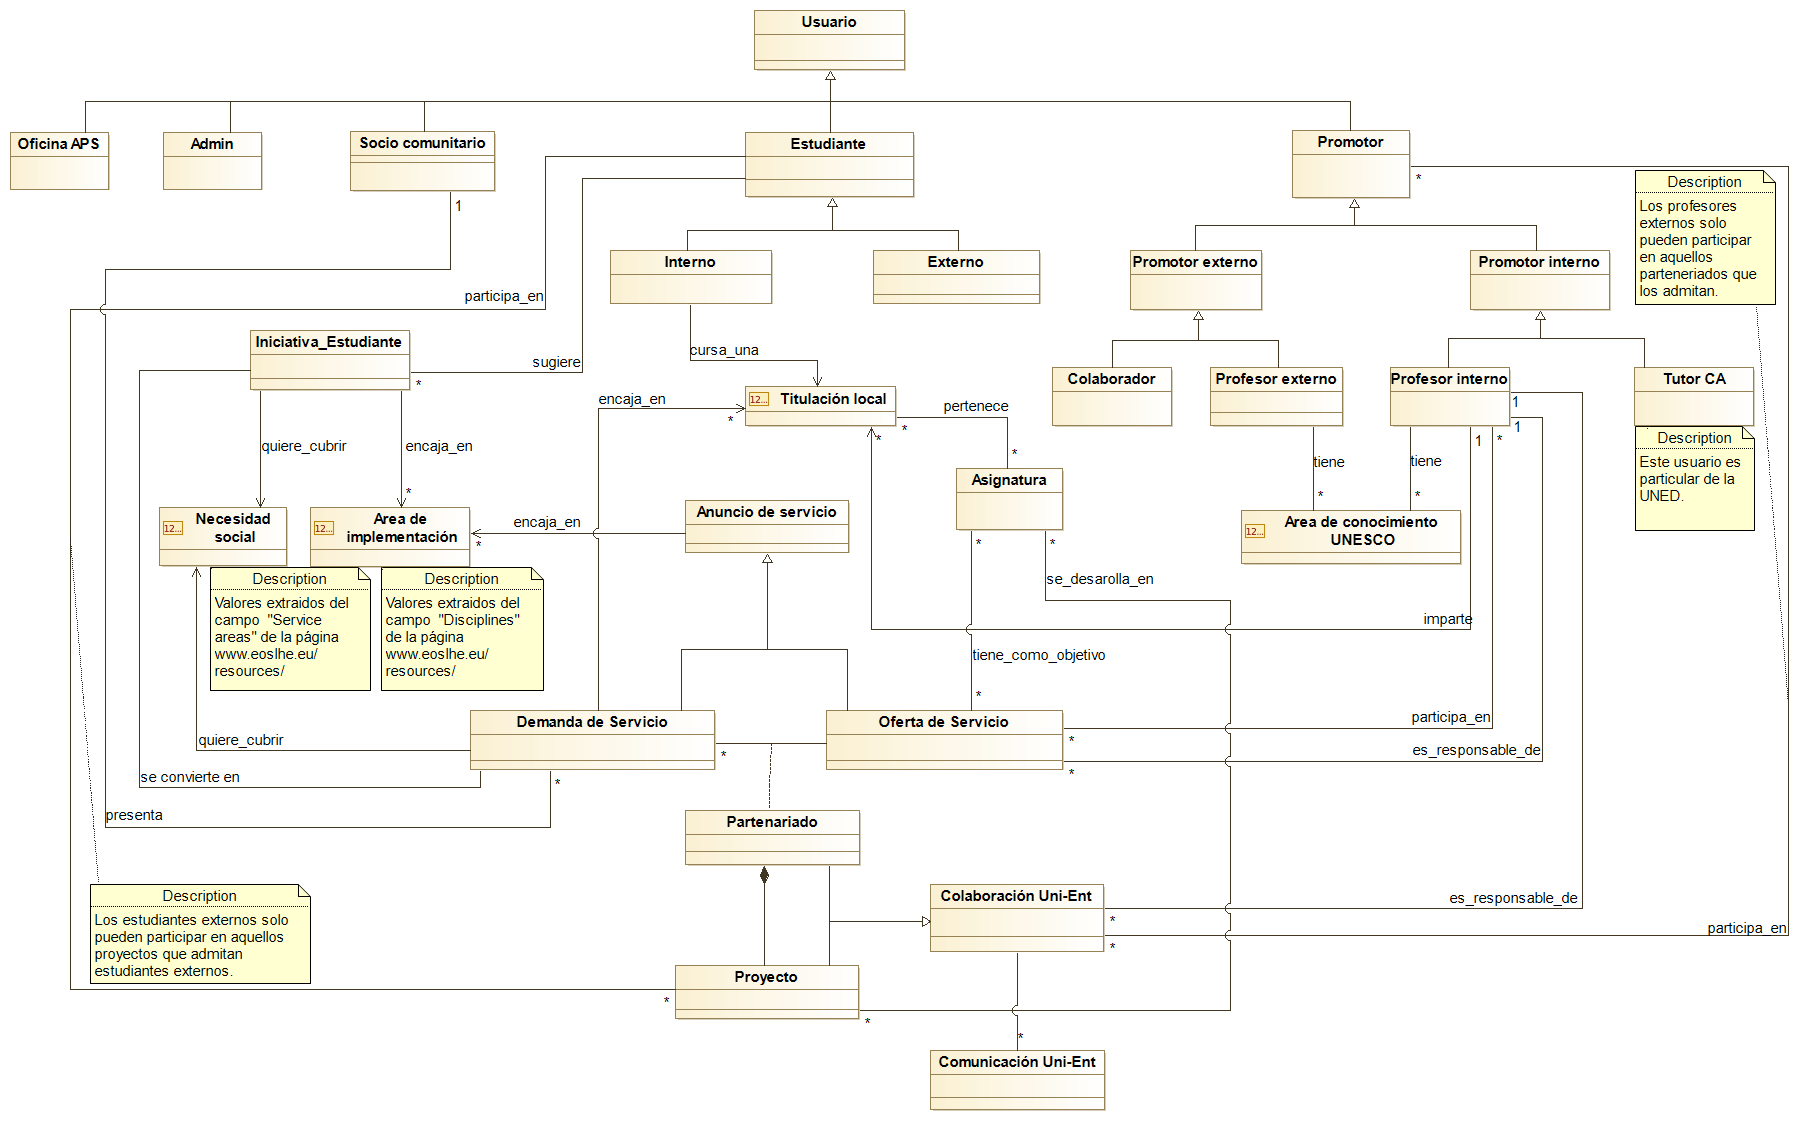
\includegraphics[scale=0.23]{mdominio}
	\caption{Modelo de dominio}
\end{figure}
\begin{figure}
	\centering
	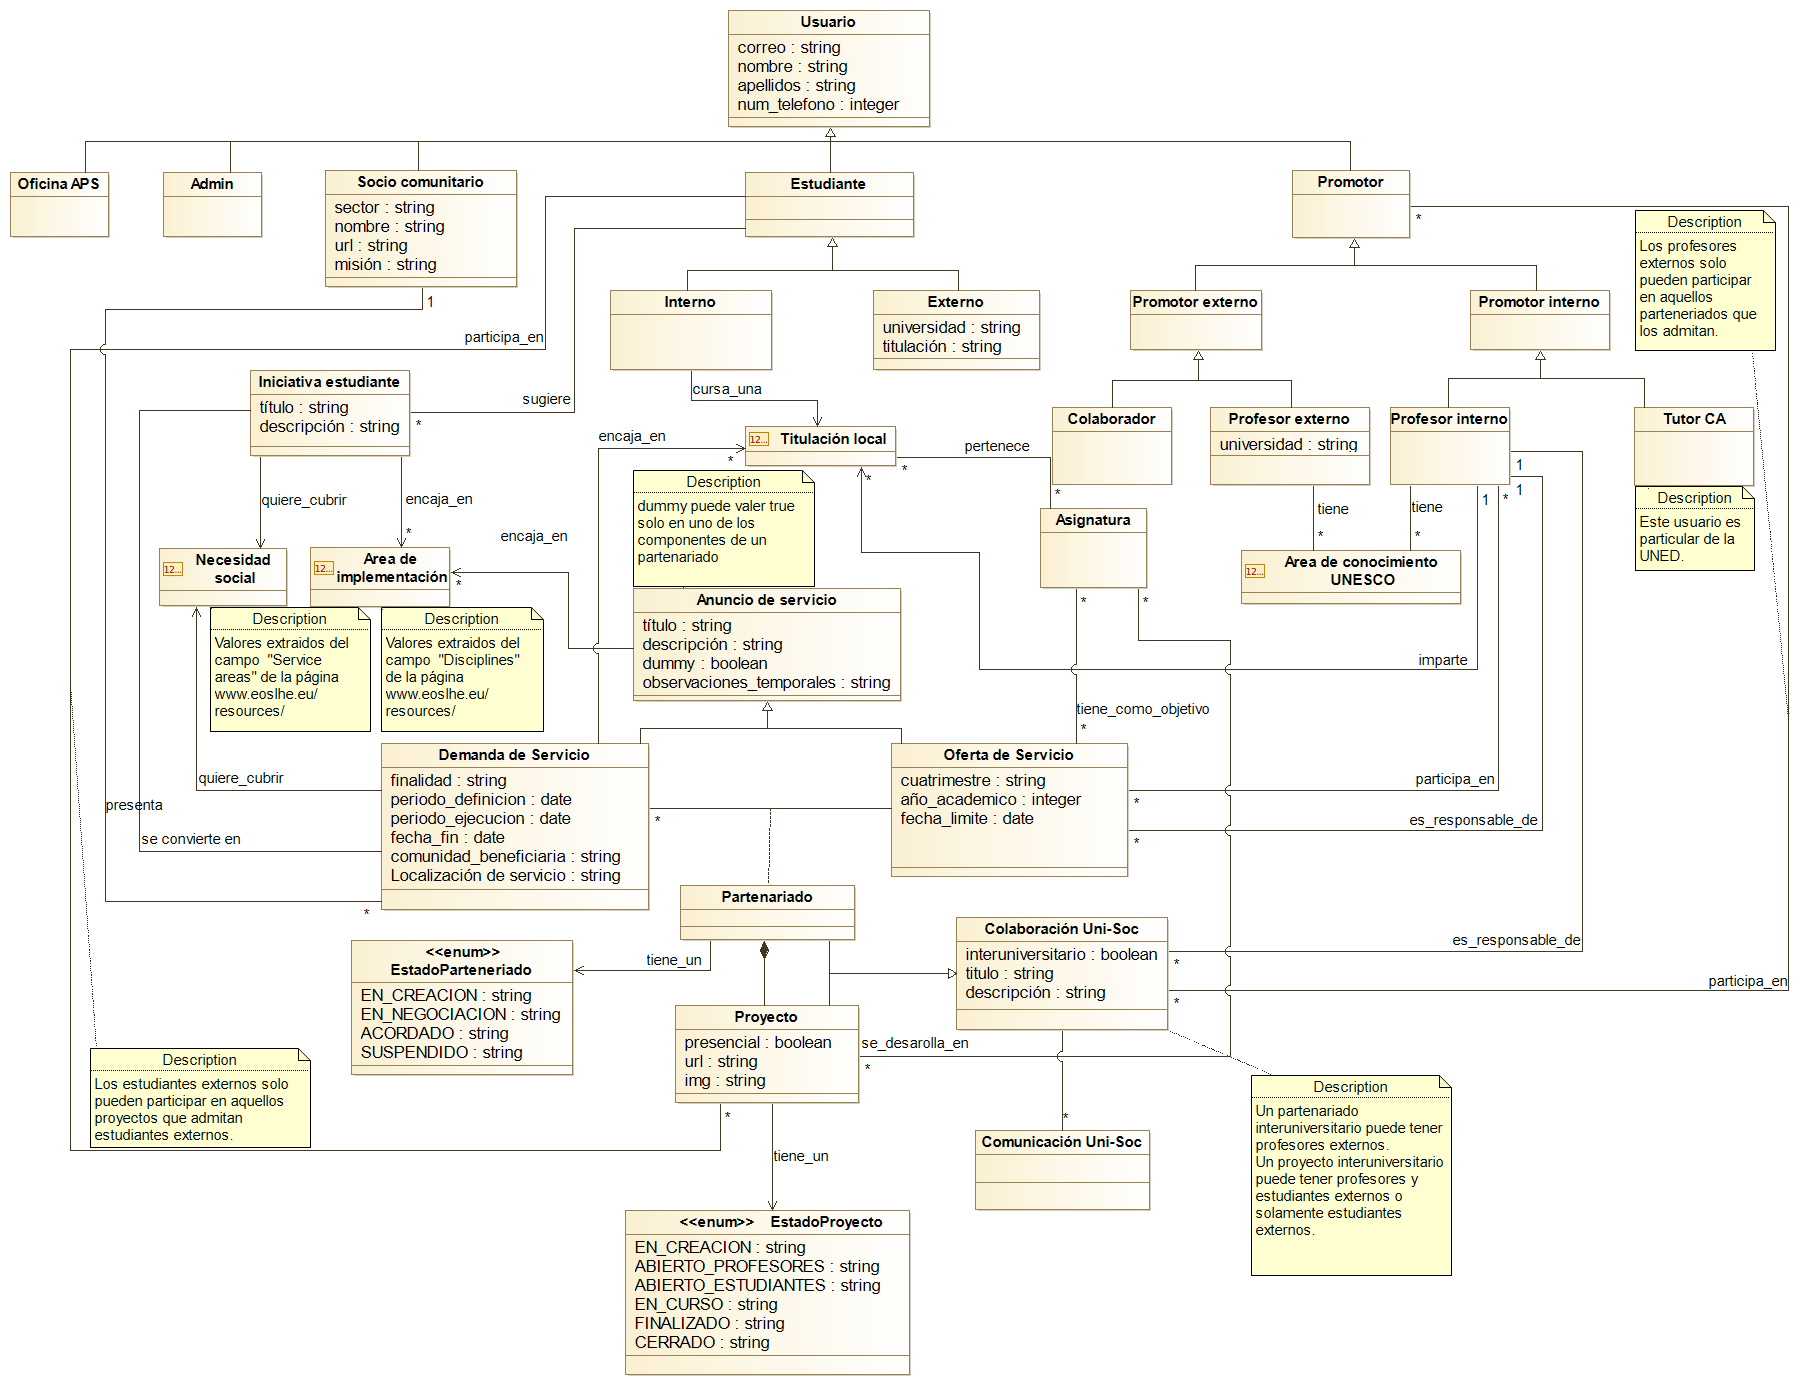
\includegraphics[scale=0.23]{mdatos}
	\caption{Modelo de datos}
\end{figure}
\subsection{Modelo de datos}
El modelo de datos describe con más precisión el dominio de la aplicación.
Además de algunos atributos importantes como el interuniversitario que indica si el partenariado o el proyecto está abierto a externos, podemos observar los estados que pueden tener el partenariado y el proyecto representados por dos enumerados.\\\\

En particular podemos ver que el partenariado puede encontrarse en estados EN\_CREACION, EN\_NEGOCIACION, ACORDADO y SUSPENDIDO.\\ 
El partenariado toma el estado de EN\_CREACIÓN cuando el profesor se pone en contacto con la entidad, si la entidad contesta y acepta aliarse con el profesor el estado del partenariado pasará a EN\_NEGOCIACION. Cuando el profesor y la entidad terminan de establecer los términos y condiciones del partenariado y ambos están de acuerdo el partenariado pasá a estar ACORDADO. Si ocurre cualquier discrepancia durante la fase de EN\_CREACION, EN\_NEGOCIACION o ACORDADO el partenariado puede pasar al estado de SUSPENDIDO.\\\\

En el caso del proyecto tenemos los estados EN\_CREACION, ABIERTO\_PROFESORES, ABIERTO\_ESTUDIANTES, EN\_CURSO, FINALIZADO y CERRADO.
Cuando el profesor decide seguir con el proyecto debe rellenar un formulario, al rellenar dicho formulario el estado del proyecto pasa a estar EN\_CREACION. La entidad recibe dicha solicitud de continuación y debe rellenar otro formulario, una vez rellenado y enviado el proyecto pasa al estado de ABIERTO\_PROFESORES. Una vez que el proyecto ha sido definido se abre a los alumnos y es allí cuando el proyecto pasa al estado de ABIERTO\_ESTUDIANTES. Si el proyecto finaliza correctamente pasará al estado de FINALIZADO. Si sucede cualquier imprevisto durante las 4 fases anteriores el proyecto puede pasar al estado CERRADO.

\subsection{Modelo relacional}

 Debido a la complejidad de la nueva base de datos compuesta por 46 tablas relacionales, se ha decidido crear un diagrama que sirva como mapa en la gestión de la base de datos.\\\\
Este modelo relacional se divide en 4 secciones claramente diferenciadas.\\
La sección de los usuarios que contiene tablas relacionadas con información de los usuarios. La sección del Anuncio de servicio que contiene todas las tablas que representan información de la oferta de servicio, la demanda de servicio y la iniciativa.
La sección de Colaboración contiene la información relacionada con el partenariado y el proyecto.
Y la última es la sección que tiene menos complejidad, la sección de Comunicación que contiene las tablas de \textit{mail}, mensaje, \textit{upload} y \textit{newsletter}, estas creadas por David que se han mantenido intactas.
\begin{figure}
	\centering
	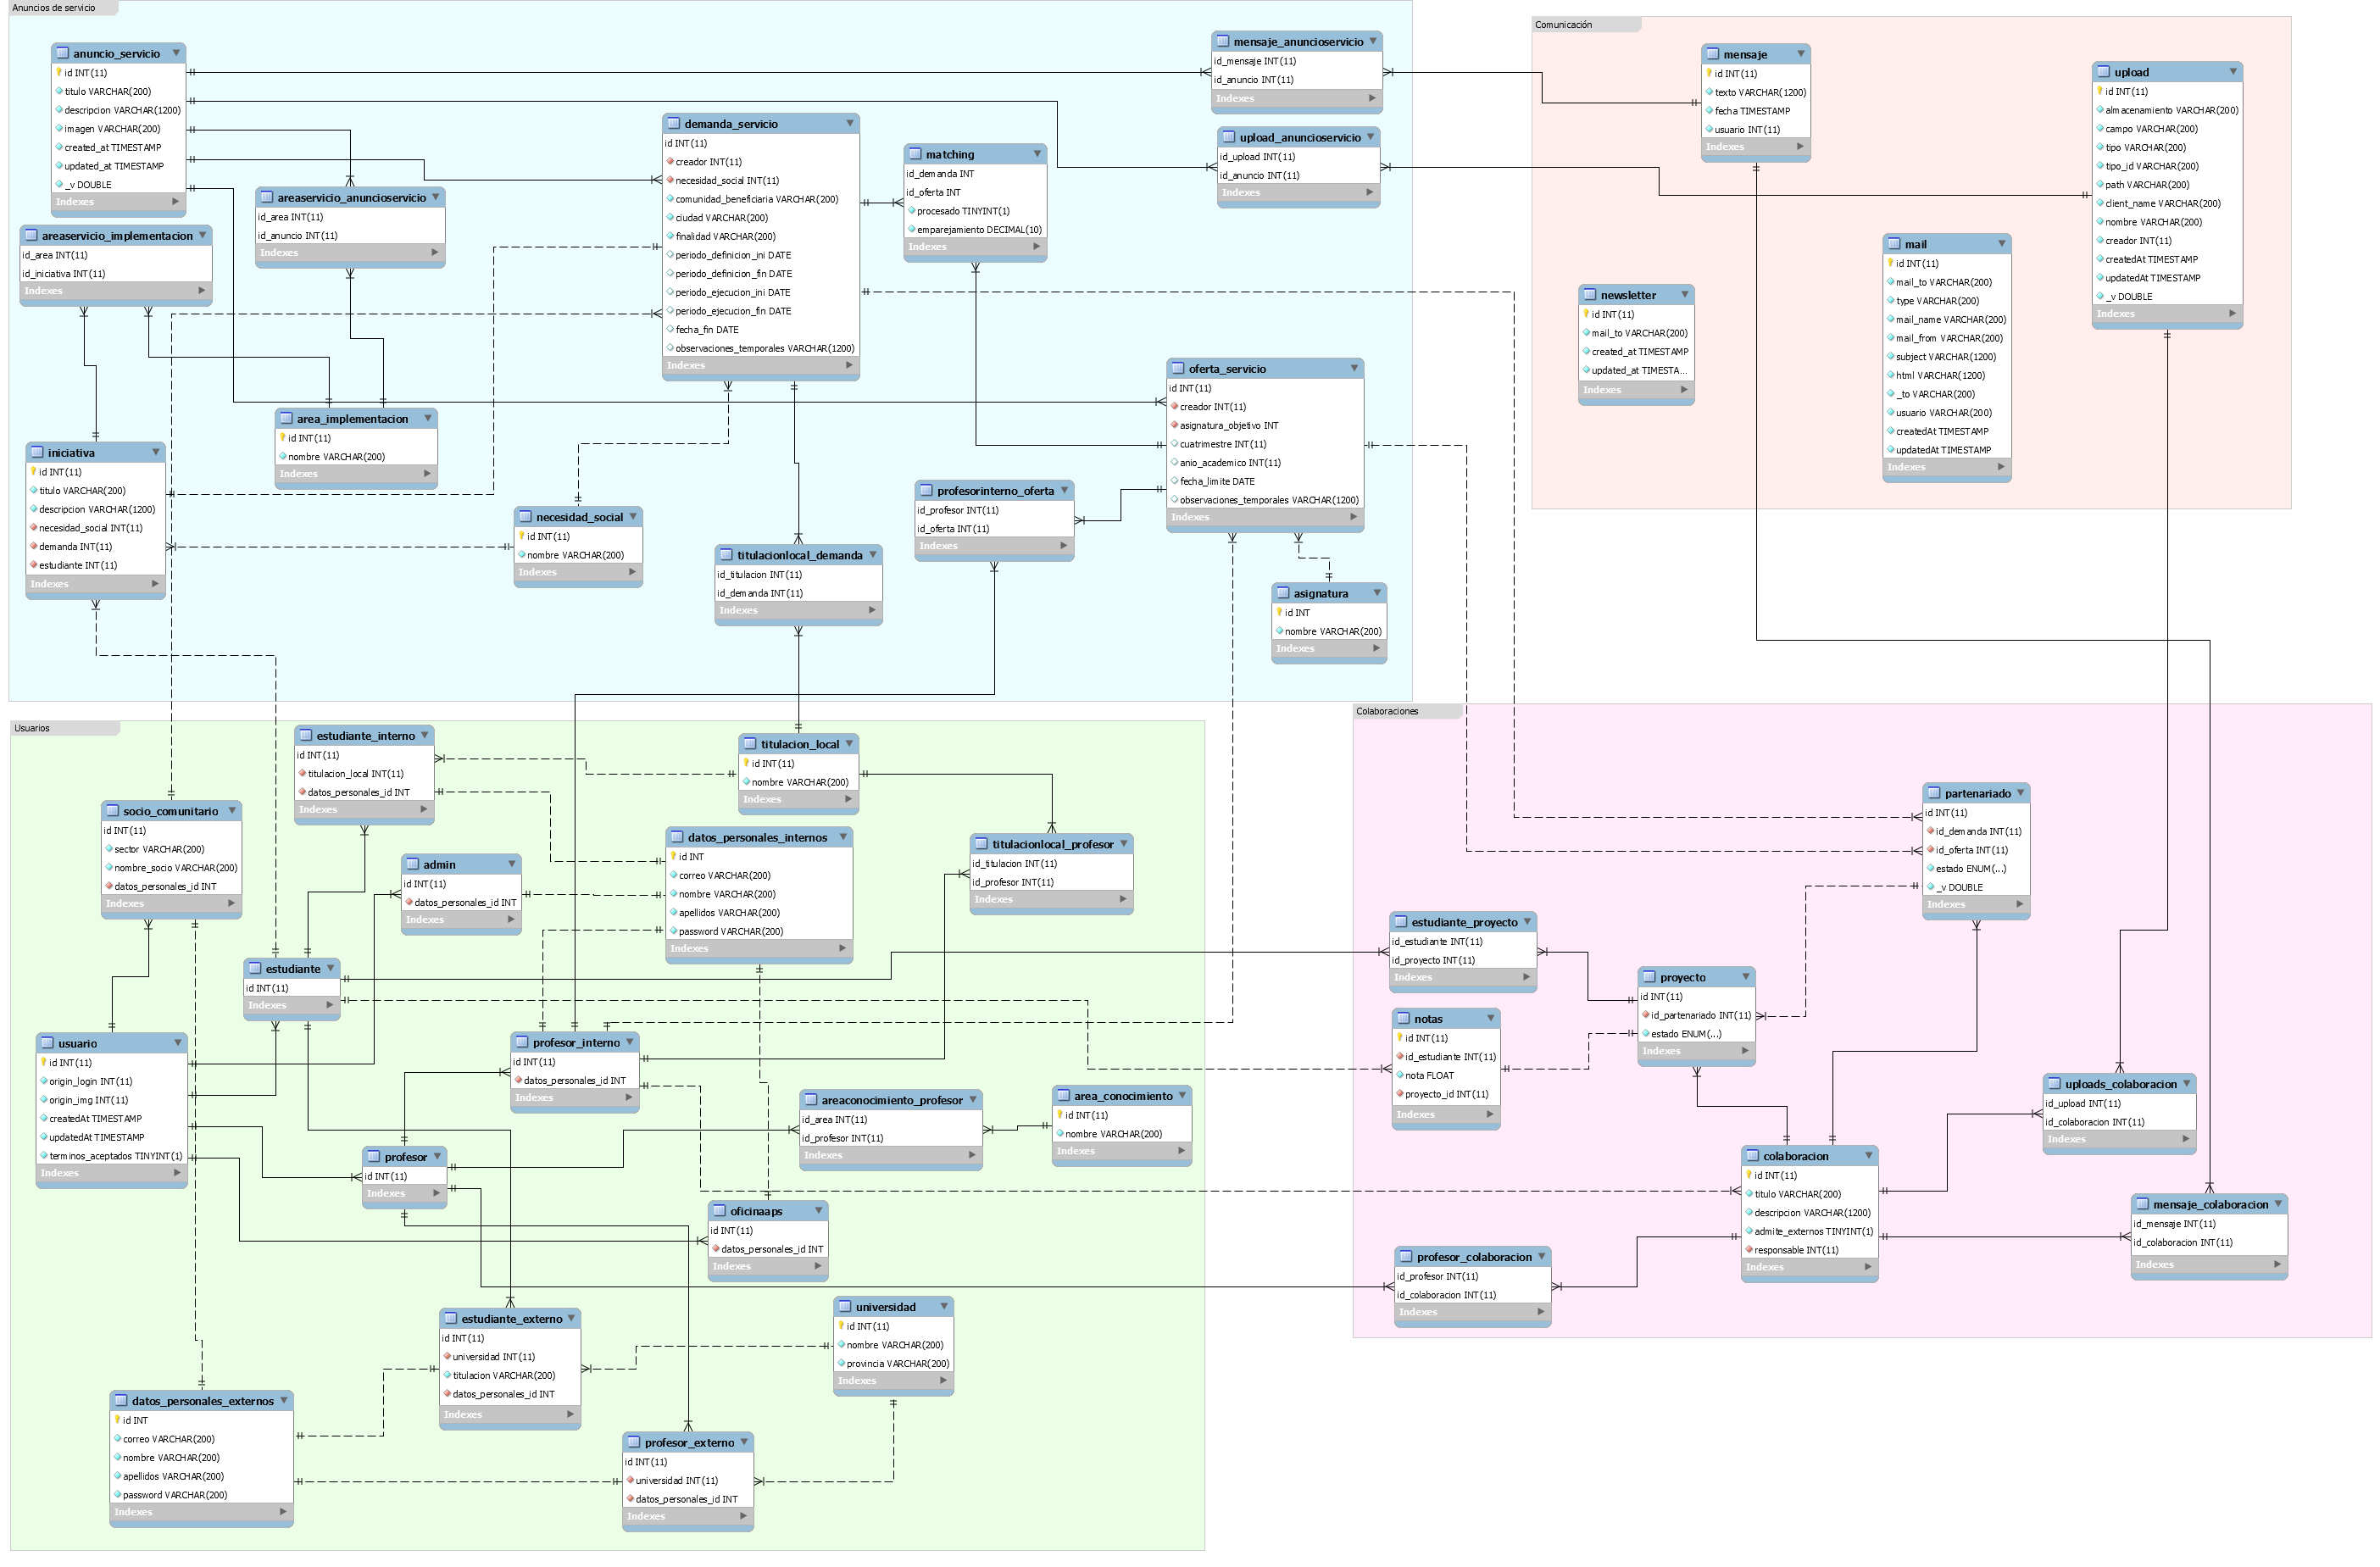
\includegraphics[scale=0.15]{er}
	\caption{Diagrama de entidad relación}
\end{figure}
\subsubsection{Usuarios}
Esta sección es la más compleja debido a la separación que hay que realizar de los usuarios externos e internos.\\
Un usuario interno es aquel profesor, tutor, colaborador, estudiante o representante de la oficina ApS que forma parte de la universidad en la que se despliega la plataforma y por tanto tiene sus datos personales dentro de ella. Debido a que estos tienen parte de los datos que necesitamos para la aplicación en el sistema interno de la universidad hay que tratarlos de manera diferente a los usuarios externos, que son aquellos que no pertenecen a la universidad. Los colaboradores y tutores que aquí mencionamos se pueden ver representados en el modelo de datos y de dominio, pero no se observan aquí porque no nos dio tiempo a integrarlos en la base de datos.\\\\
Debido a esta separación, todos los usuarios comparten una tabla común llamada usuario que contiene datos exclusivos de la cuenta de la plataforma. Después tenemos tablas que contienen datos particulares de cada tipo de usuario, estas son las tablas de entidad, estudiante interno, estudiante externo, \textit{admin}, profesor interno, profesor externo y oficina ApS.\\
Cada uno de estos usuarios poseen una tabla que almacena sus datos personales haciendo diferenciación entre internos y externos. La tabla de datos\_personales\_internos es una tabla creada para la simulación de la aplicación, una vez la aplicación sea desplegada en un entorno real esta tabla será eliminada y los datos personales se obtendrán haciendo consultas a la base de datos de la universidad.\\
Después podemos observar tablas secundarias que representan características de los usuarios como es, la universidad del profesor y estudiante interno, las Áreas de Conocimiento UNESCO de los profesores y las titulaciones que imparten los profesores o cursan los alumnos.
\begin{figure}
	\centering
	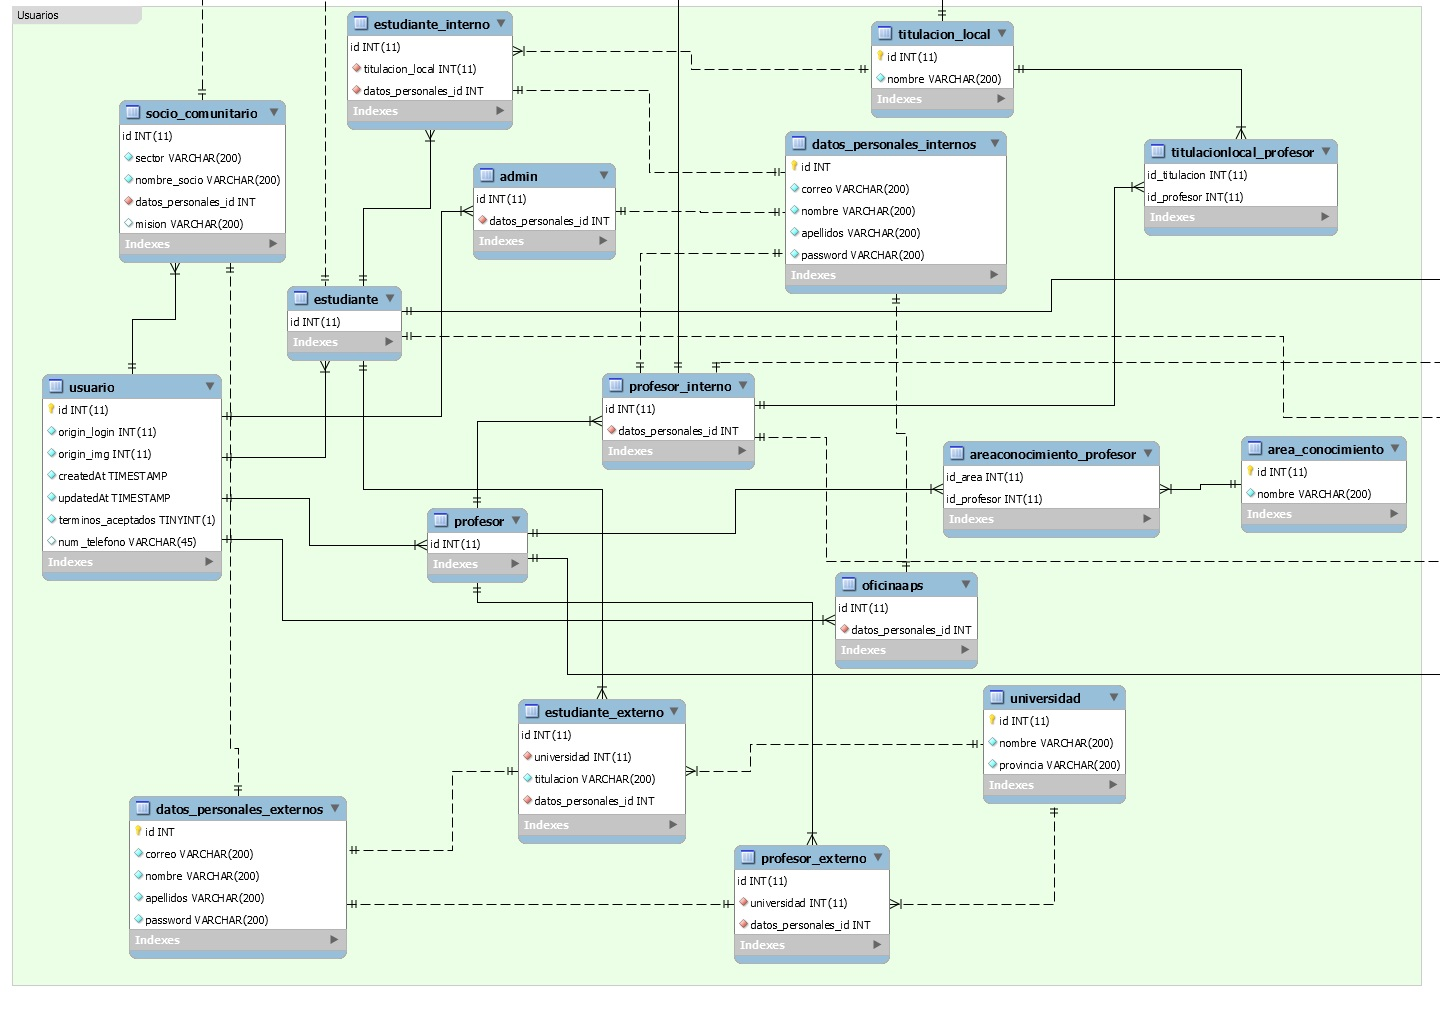
\includegraphics[scale=0.4]{usuarios}
	\caption{Diagrama de entidad relación: Usuarios}
\end{figure}
\subsubsection{Anuncios de servicio}
En este conjunto de tablas podemos encontrar las pertenecientes a la demanda de servicio, la oferta de servicio y la iniciativa.\\
La iniciativa es una propuesta de proyecto realizada por un estudiante. Esta propuesta debe ser validada por un administrador y posteriormente adoptada por una entidad que desee realizar el proyecto.\\\\
La demanda de servicio es creada por una entidad y define una necesidad especifica que quiere cubrir. Esta necesidad social es representada por un enumerado alojado en la tabla de necesidad\_social.
Estos enumerados han sido obtenidos del campo Service areas hallado en la página www.eoslhe.eu/resources/ .
Los enumerados alojados en la tabla area\_servicio también se obtuvieron de esta página, del campo llamado Disciplines.\\\\
La oferta de servicio es creada por un profesor interno y tiene menos detalles que la demanda porque es una propuesta más genérica.\\
Cuando una oferta y una demanda son procesadas por el sistema de \textit{matching} se crea una entrada en la tabla \textit{matching} almacenando los \textit{ids} de ambos elementos y el porcentaje de emparejamiento que tienen.\\
Tanto demanda de servicio como oferta de servicio están conectadas a mensajes y \textit{uploads} porque estos permiten la comunicación con las personas interesadas en las propuestas.
\begin{figure}
	\centering
	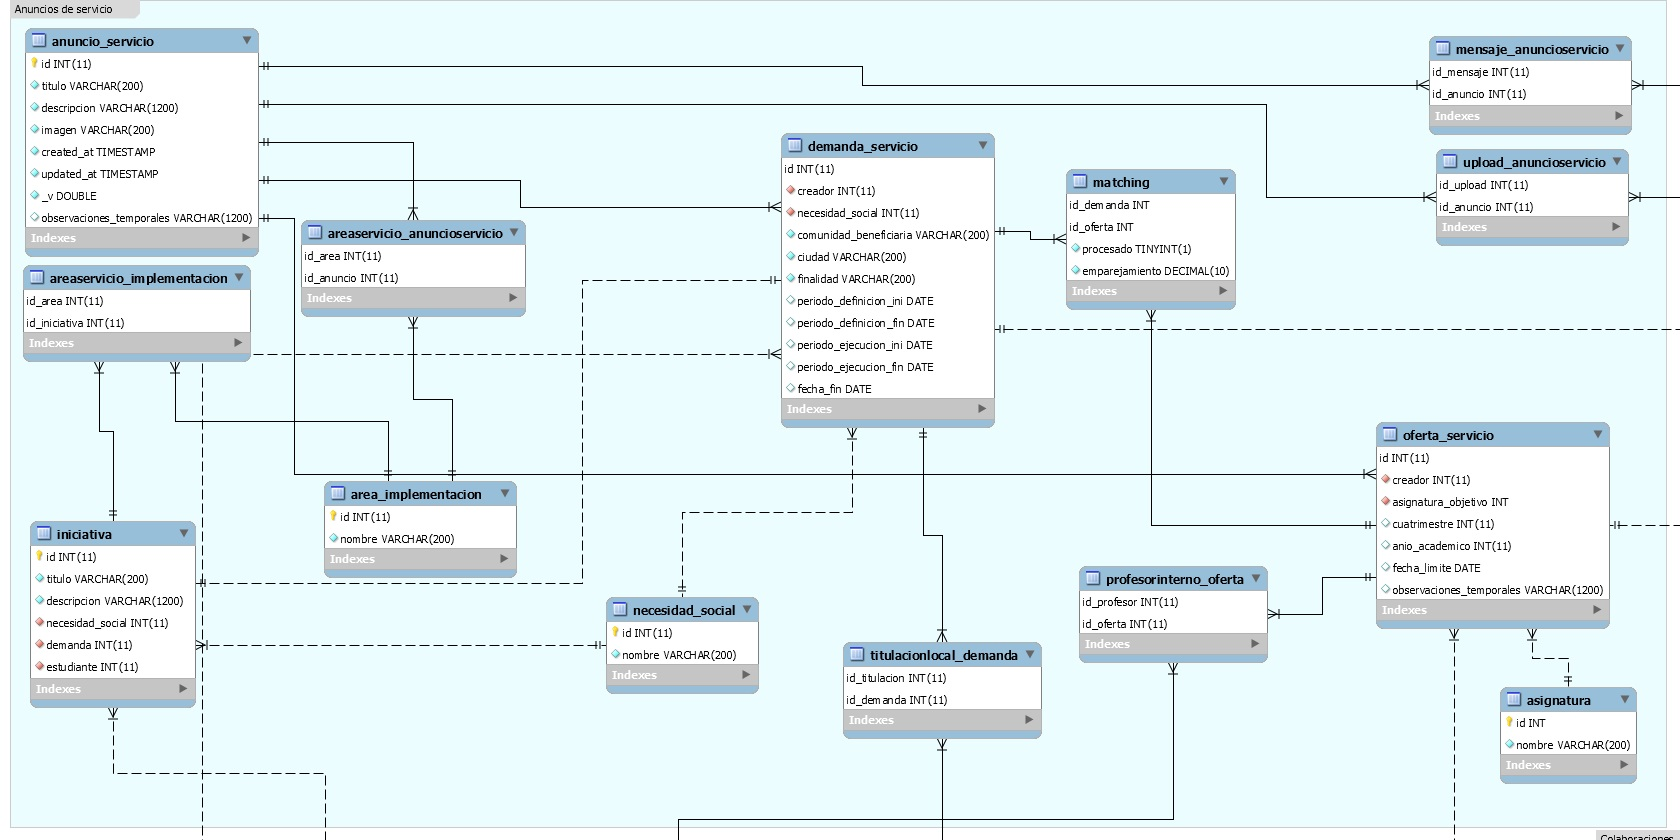
\includegraphics[scale=0.35]{anuncios}
	\caption{Diagrama de entidad relación: Anuncios de servicio}
\end{figure}
\subsubsection{Colaboración}
El partenariado es el segundo paso en la creación de un proyecto, esta tabla contiene las \textit{ids} de la demanda y la oferta que la componen.\\
El proyecto no puede existir sin un partenariado y es por eso por lo que tiene un id del partenariado que lo creó. El proyecto posee estudiantes y es por eso por lo que tiene una conexión con los mismos.\\
Tanto proyecto como partenariado necesitan un sistema de comunicación y es por eso por lo que tienen tablas intermedias que los conectan a mensaje y \textit{uploads}.
\begin{figure}
	\centering
	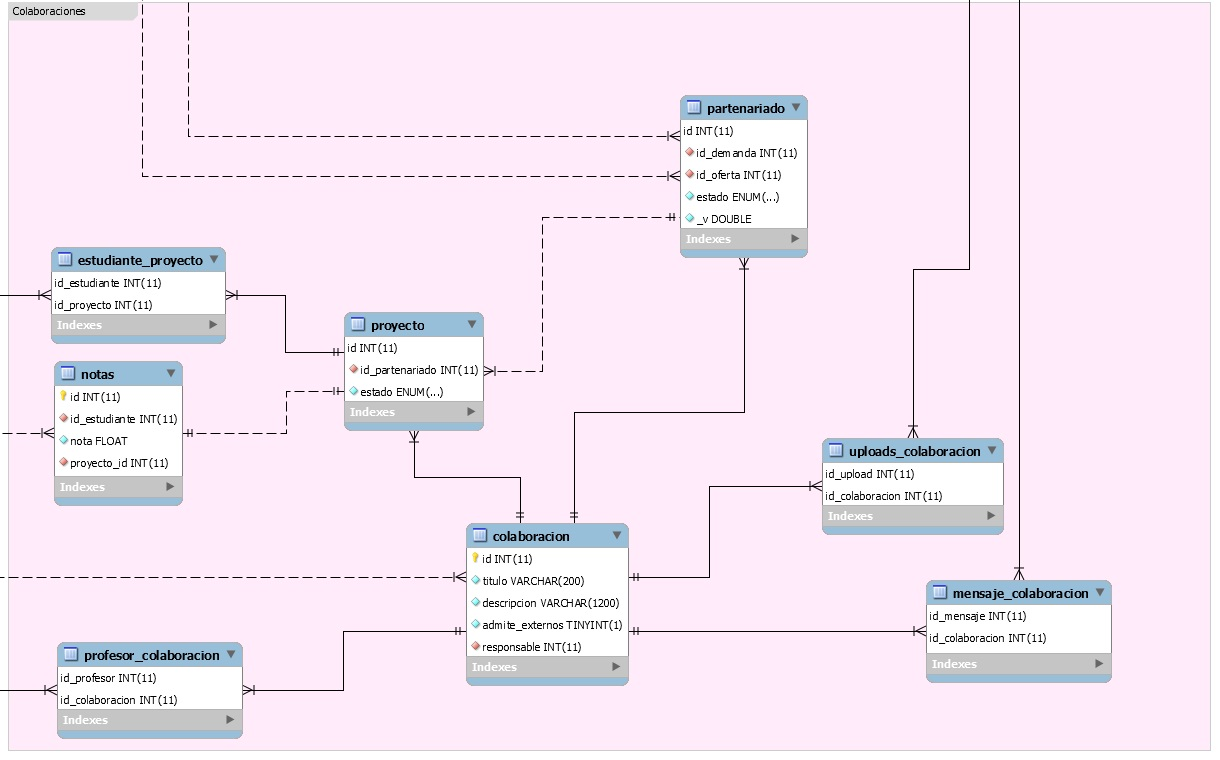
\includegraphics[scale=0.4]{colaboracion}
	\caption{Diagrama de entidad relación: Colaboración}
\end{figure}
\subsubsection{Comunicación}
Esta parte se ha mantenido tal y como la había creado David, solo se ha adaptado al nuevo sistema.\\
La tabla de mensajes conecta con las ofertas de servicio, las demandas de servicio, los partenariados y los proyectos porque todos estos necesitan de los mensajes para poder comunicarse.\\
La tabla \textit{upload} almacena la información de los ficheros e imágenes subidos tanto en ofertas de servicio, como demandas de servicio, como partenariados y proyectos.\\
La tabla \textit{mail} y \textit{newsletter} no han sido conectadas con nada porque no se han tenido en cuenta para el desarrollo de este TFG pero representan los correos electrónicos internos de la aplicación y las noticias periódicas enviadas a los usuarios.
\begin{figure}
	\centering
	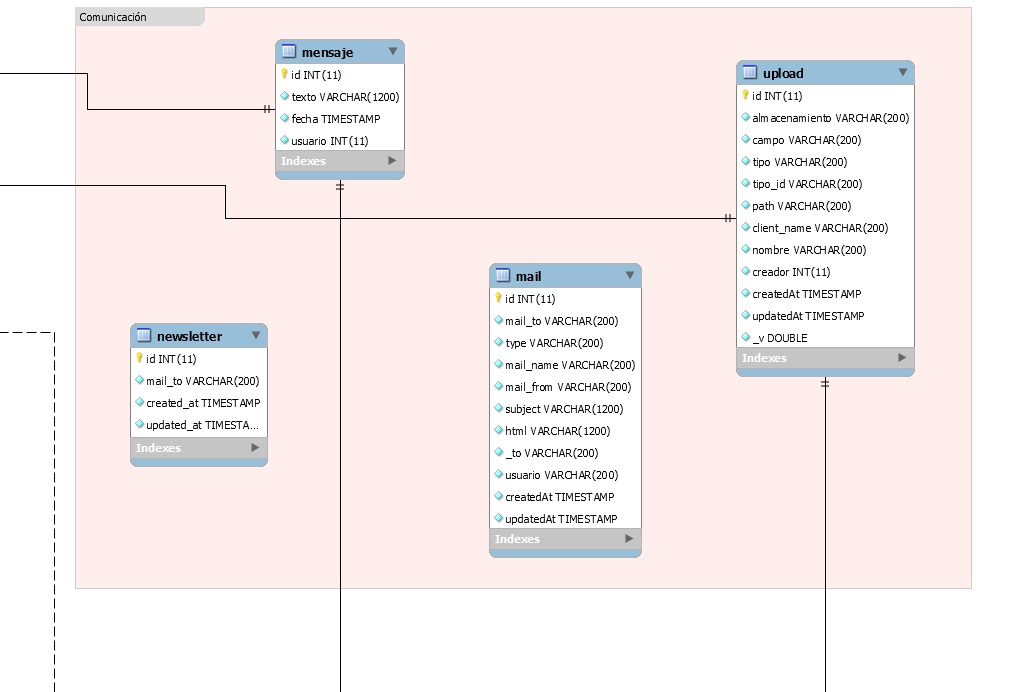
\includegraphics[scale=0.4]{comunicacion}
	\caption{Diagrama de entidad relación: Comunicación}
\end{figure}

\bibliographystyle{plain}
\bibliography{references}
\end{document}